\section{Exercise 1: Entropy of a Random Variable with 3 Outcomes}

\begin{frame}{Entropy and Probability Vectors}
In this exercise, we analyzed the entropy of a random variable with three possible outcomes. The entropy \( H(p) \) is defined as:

\[
H(p) = - \sum_{i=1}^3 p_i \log_2 p_i
\]

where \( p = [p_1, p_2, p_3] \) represents the probability vector for the outcomes. The goal was to:
\begin{itemize}
    \item Calculate entropy over the probability simplex.
    \item Apply an iterative averaging procedure to observe entropy evolution toward uniformity.
    \item Show that entropy approaches its maximum as the distribution becomes uniform.
\end{itemize}
\end{frame}

\begin{frame}{Entropy over the Probability Simplex}
We generated all valid probability vectors where \( p_1 + p_2 + p_3 = 1 \) and \( p_i \geq 0 \), and computed the entropy for each. The highest entropy occurs when the probabilities are equally distributed (\( p_1 = p_2 = p_3 \)).

\vspace{3mm}  % Add vertical space between the text and the graph

\begin{figure}[ht]
    \centering
    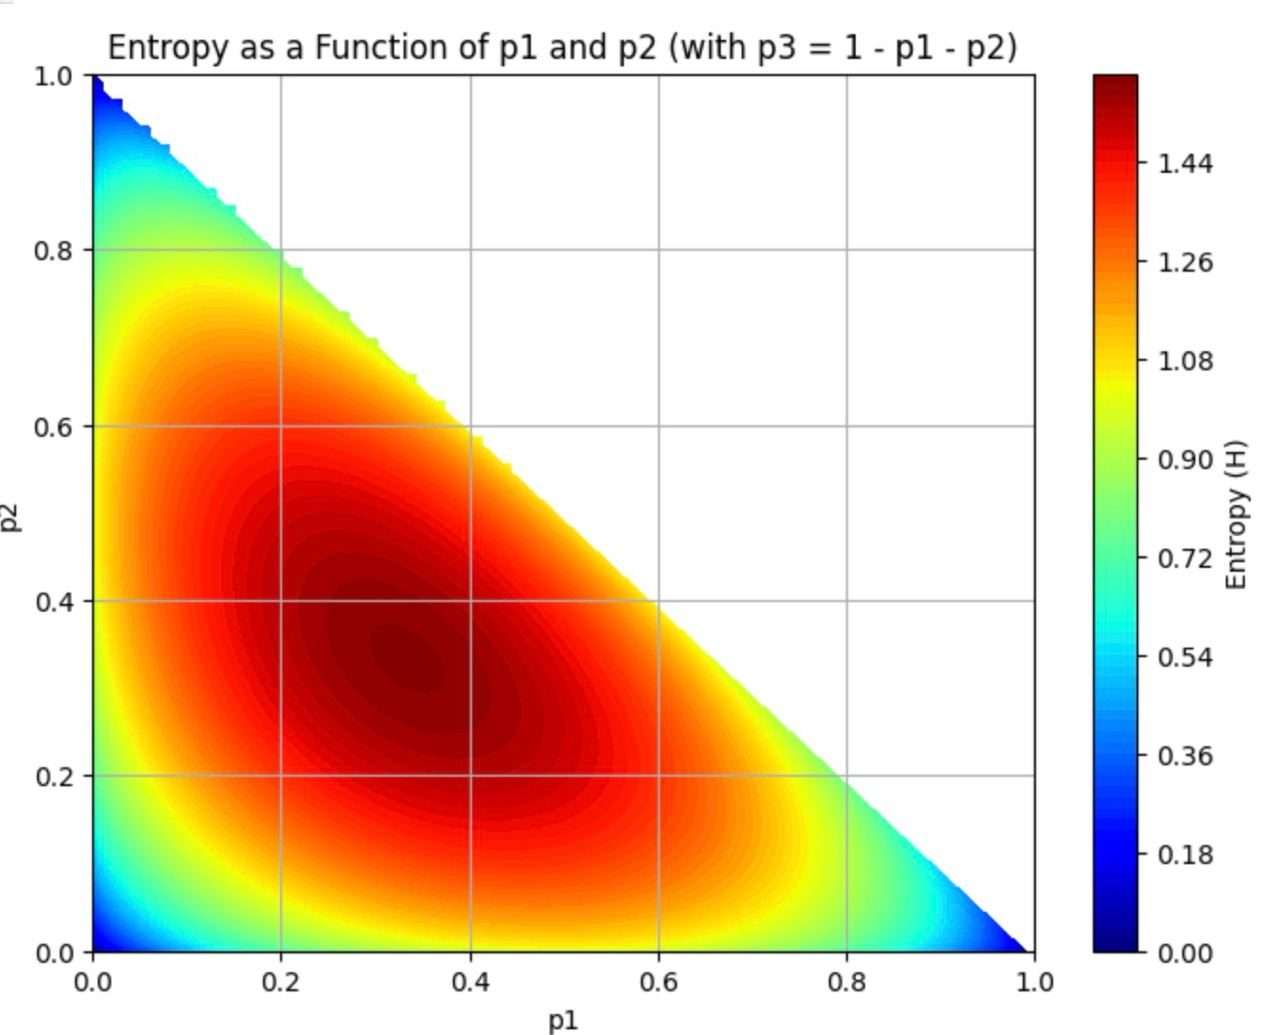
\includegraphics[width=0.4\textwidth]{images/2.jpg}
    \hspace{5mm}
    \parbox[b]{0.3\textwidth}{\caption{Figure 1: Entropy across the probability simplex. Highest entropy at uniform distribution.}}  % Correct the double "Figure" issue
    \vspace{-5mm}  % Bring the caption closer to the graph
\end{figure}
\end{frame}


\begin{frame}{Iterative Averaging Procedure}
We started with a skewed probability vector \( p = [0.98, 0.01, 0.01] \) and applied an iterative averaging procedure. Probabilities were updated and normalized after each iteration, demonstrating how the distribution evolves towards uniformity.

\vspace{3mm}  % Add vertical space between the text and the graph

\begin{figure}[ht]
    \centering
    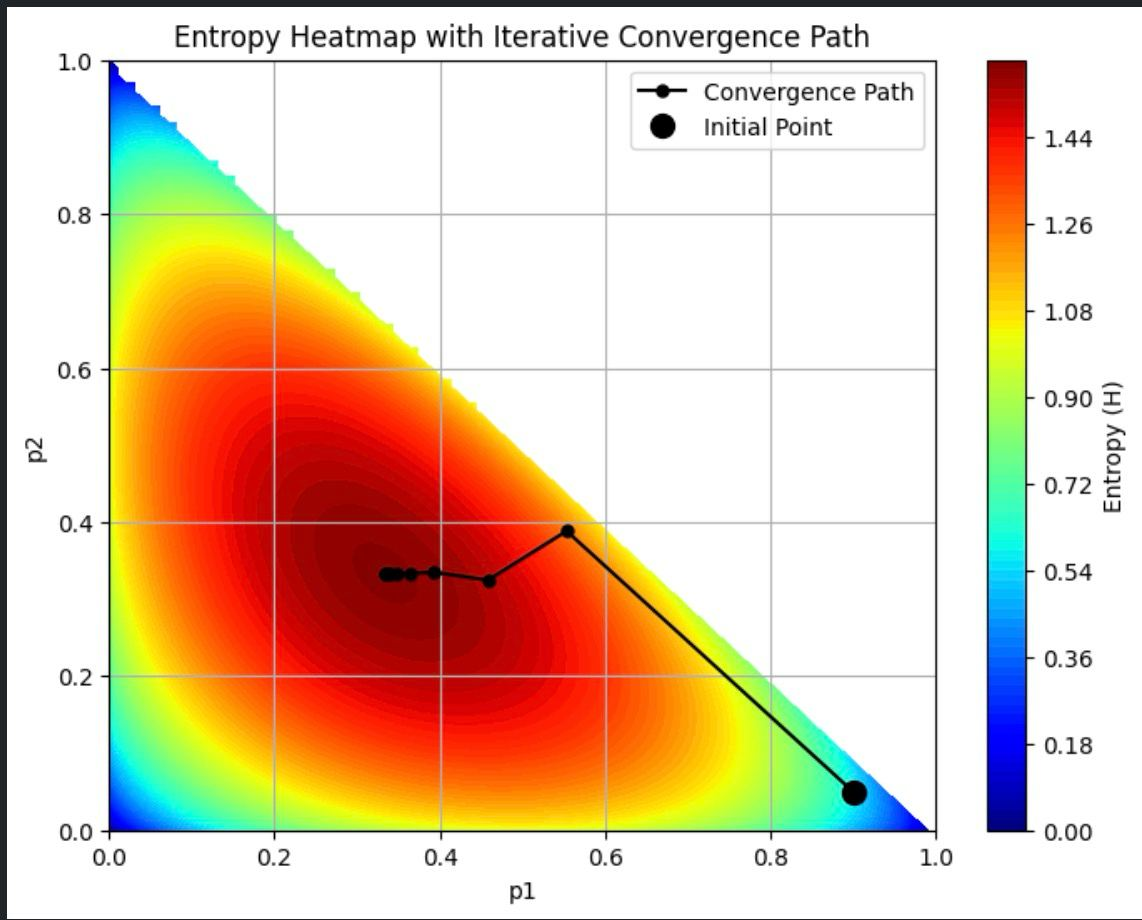
\includegraphics[width=0.4\textwidth]{images/1.jpg}
    \hspace{5mm}
    \parbox[b]{0.3\textwidth}{\caption{Figure 2: Entropy evolution during iterative averaging. Entropy rises as the distribution balances.}}  % Correct the double "Figure" issue
    \vspace{-5mm}  % Bring the caption closer to the graph
\end{figure}
\end{frame}

\begin{frame}{Results and Conclusion}
In this exercise, we:
\begin{itemize}
    \item Calculated entropy over the probability simplex, confirming that entropy is maximized when probabilities are uniformly distributed.
    \item Applied an iterative averaging process starting with a skewed probability vector. Each iteration brought the distribution closer to uniformity, with the corresponding entropy values increasing, approaching the theoretical maximum.
    \item Visualized the convergence of the entropy values as the probability vector approached uniformity.
\end{itemize}

Overall, the experiment demonstrated the direct relationship between entropy and distribution balance: skewed distributions have low entropy, while uniform distributions achieve maximum entropy. The iterative procedure successfully illustrated how entropy evolves as randomness in the distribution increases.
\end{frame}
